\section{Introduction}\label{sec:intro}

Neural surrogates of finite-element models return, in one network evaluation, the field that
an assembly and a solve would return, so that design studies and uncertainty quantification
can query many configurations cheaply
\cite{Pfaff2021,Lu2021DeepONet,Li2021FNO,He2024GeomDeepONet,Zeng2025PCNO,Liu2026GINOT}. They
are usually trained by minimising a mean-square or relative error of the displacement
against reference solutions, and compared by the same error. Both choices fix a norm, the
Euclidean norm of the nodal displacements, and neither is usually discussed. The stresses,
on which engineering decisions depend, are measured by another norm. This paper shows that,
for the surrogates we trained, the choice of norm decided their stress accuracy more than
whether solutions were used at all.

The clearest symptom is a reversal. A transformer trained on the discrete potential energy
of 1,024 three-dimensional instances, without a single solve, had lower displacement, energy
and stress errors, in each of three seeds, than the same transformer trained on the exact
solutions of the same instances, some of whose predictions were worse than the zero field.
Reported comparisons of energy-trained and supervised networks disagree: the two were about
as accurate in one study \cite{Zhu2019}, the energy-trained network was the more accurate in
energy, strain or stress in two others \cite{Dalton2023,MonteiroFernandes2025}, and the less
accurate in a third \cite{Sun2026FEVessel}.

The explanation is a classical identity. The energy of a prediction exceeds that of the
solution by half its squared error in the energy norm \cite{Ciarlet1978}, which is the
strain energy of its stress error. Minimising the energy over a training set is therefore
exactly supervised regression in the energy norm, with the same gradients, although no
solution is computed. Minimising the displacement error is regression in the Euclidean norm,
which weights all eigenmodes of the stiffness matrix equally and so under-weights the stiff
modes that carry the strains; a Euclidean residual loss regresses in the norm of the squared
stiffness matrix. Supervision and energy training thus differ, before anything else, in the
norm they minimise.

We test this by separating the norm from the labels (\cref{fig:normlabels}). The same
network, on the same instances, is trained on the solutions in the Euclidean norm, on the
solutions in the energy norm, and without solutions in the energy norm; the fourth
combination does not exist, because a displacement loss needs the solutions. Removing the
solutions also changes the weighting of the load cases and the learning rate
(\cref{sec:labelfree}). In three dimensions, changing the norm with the labels kept cut the
median energy-norm error \numNlThreeNormE{}-fold and the median von Mises error
\numNlThreeNormVm{}-fold; removing the labels with the energy norm kept raised them by
factors of \numNlThreeLabelE{} and \numNlThreeLabelVm{}. In two dimensions the energy norm
more than halved the von Mises error of supervision. On the means over the instances,
changing the norm divided the energy-norm and von Mises errors by \numNlThreeNormEMean{} and
\numNlThreeNormVmMean{} in three dimensions and by \numNlCmNormEMean{} and
\numNlCmNormVmMean{} in two. The comparisons were pre-registered (\cref{tab:claims}), and
their claims were read again on held-out instances.

\begin{figure}[tbp]
\centering
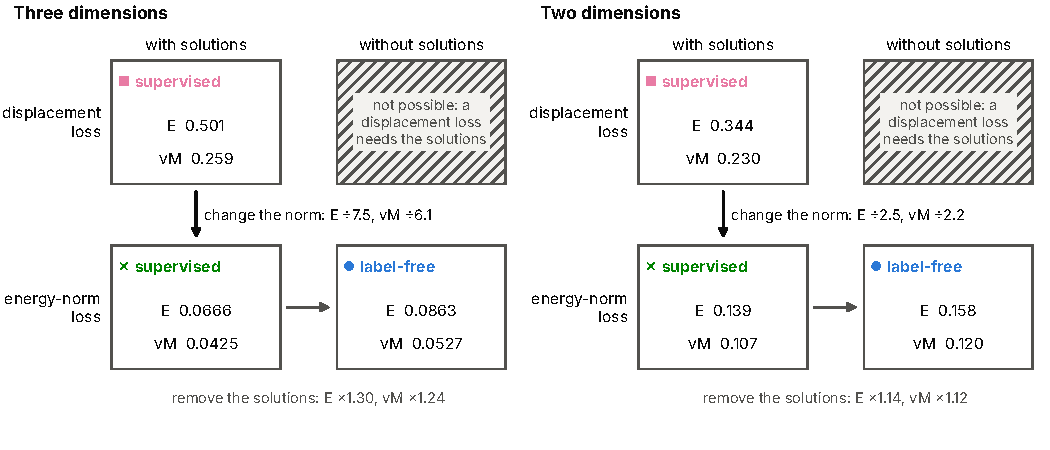
\includegraphics[width=\linewidth]{generated/fig_norm_labels.pdf}
\caption{The norm of the loss against the labels, in three dimensions (left) and two (right).
The same transformer is trained on the solutions of 1,024 instances with the relative
displacement error (top left) or the relative energy-norm error (bottom left), and on the
energy of the same instances without their solutions (bottom right); a displacement loss
needs the solutions (top right). E: relative energy-norm error; vM: relative von Mises
error; medians over the 256 validation instances, averaged over three seeds.}
\label{fig:normlabels}
\end{figure}

The norm matters for evaluation as well. Ranked by displacement error, a graph network
trained on the solutions was the most accurate of the three-dimensional networks; ranked by
von Mises error, it was among the least accurate, at \numThreeMgnOverFreeVm{} times the
label-free transformer's. The energy itself checks predictions without a solution:
differences of energy rank the predictions of a load case by their energy-norm errors, and
the sign of the energy shows whether a prediction is worse than the zero field. A posteriori
error estimators bound the energy-norm error itself, at the price of an equilibrated stress
field or a few Krylov iterations (\cref{sec:related}); these two checks need neither.

We do not claim that the networks beat classical methods on these problems. Given the
stiffness matrix, a polynomial Ritz projection with \numRitzThreeKMax{} unknowns was more
accurate than the label-free transformer, in the seed means, on every metric but peak
stress, and conjugate gradients reached a network's accuracy within a few times its
inference time (\cref{sec:cost}). Linear elastostatics is the setting in which the identity
is exact and the comparison can be kept narrow. Its lesson, the choice of norm, should
matter wherever surrogates are trained and compared; training without solutions pays most
where solves are expensive.

The contributions are three. First, an exact account of what three common losses regress on
the assembled system (\cref{sec:theory}): the energy, in the energy norm, which bounds the
von Mises error for a homogeneous isotropic material; the displacement error, in the
Euclidean norm; and the Euclidean residual, in the norm of the squared stiffness matrix. A
spectral factor relates the energy-norm and the displacement errors and shows when they rank
predictions in opposite orders. Second, a controlled separation of the norm of the loss from
the labels in two and three dimensions (\cref{sec:norm,sec:labelfree}), with criteria fixed
before the runs and read again on held-out instances (\cref{sec:holdout}), where seven of
eight claims replicated and one, the two-dimensional reduction of the mean energy gap, did
not. Third, evidence that displacement errors misrank surrogates by stress, and two checks
that need no solution, with a closed-form rescaling for predictions that fail them
(\cref{sec:checks}). A classical baseline and the cost of each step (\cref{sec:cost}) bound
these claims. The identity, the conditioning bounds of \cref{sec:theory} and their
executable checks were first stated in a companion note \cite{CaoSong2026}.
